\documentclass[10pt,a4paper,twocolumn]{article}
\usepackage{media9}
\usepackage[utf8]{inputenc}
\usepackage[T1]{fontenc}
\usepackage[czech]{babel}
\usepackage{graphicx}
\usepackage[left=1.8cm,text={18cm, 25cm},top=1.8cm]{geometry}
\title{Signály a systémy}
\author{Martin Pech\\xpechm00@stud.vutbr.cz}

\begin{document}
	\begin{titlepage}
	\begin{center}
		\Huge
		\textsc{Vysoké učení technické v Brně\\ Fakulta informačních technologií} \\[70mm]
		\LARGE
		Signály a systémy - projekt\\
		Filtrování signálu\\
		
		\Large Řešeno pomocí jazyka \textbf{Python}\\[130mm]
		{\Large 2021 \hspace{108mm}Martin Pech (xpechm00)}
	\end{center}
	\end{titlepage}



	\section{Zpracování signálu}
	Vstupní signál jsem načetl pomocí funkce \texttt{wavfile.read} z knihovny \texttt{scipy.io}.
	Délka načteného signálu ve vzorcích činila \textbf{43316} vzorků. S pomocí vzorkovací frekvence jsem spočítal, že tato délka odpovídá času \textbf{2.70725} sekundy.
	\begin{itemize}
	\item Minimální hodnota vzorku činí: \textbf{-1572}
	\item Maximální hodnota: \textbf{2308}
	\end{itemize}
	\hspace*{-1cm}  
	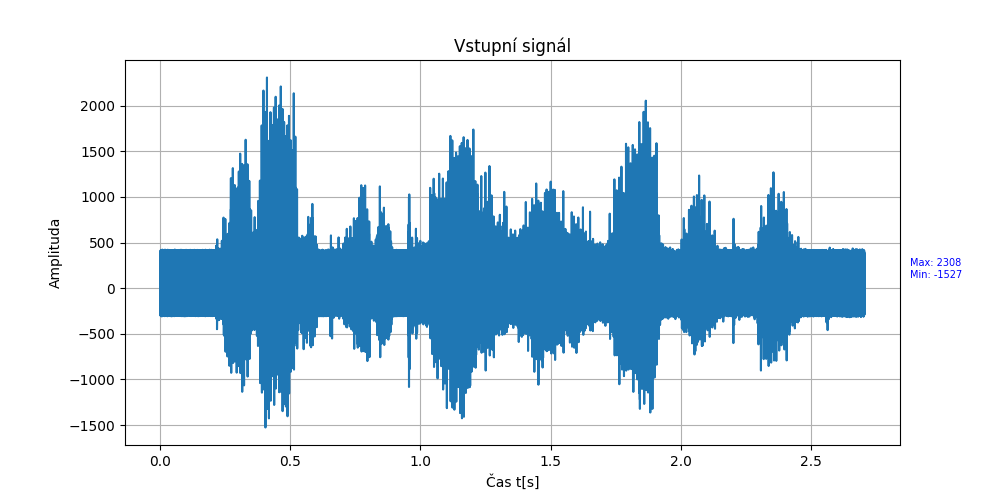
\includegraphics[scale=0.37]{Figure_1}
	
	\section{Předzpracování a rámce}
	Vytvořil jsem si funkci pro ustředění signálu. Po provedení dojde k ověření, že se signál skutečně normalizoval. V případě úspěchu i neúspěchu dojde k vypsání informace.
	
	Pro rozdělení signálu na rámce jsem implementoval vlastní funkce, i když vím, že existují podobné funkce v knihovně \texttt{scipy}. Jako \textit{pěkný} rámec jsem zvolil rámec číslo \textbf{35}, který je krásně periodický.
	\hspace*{-1cm}
	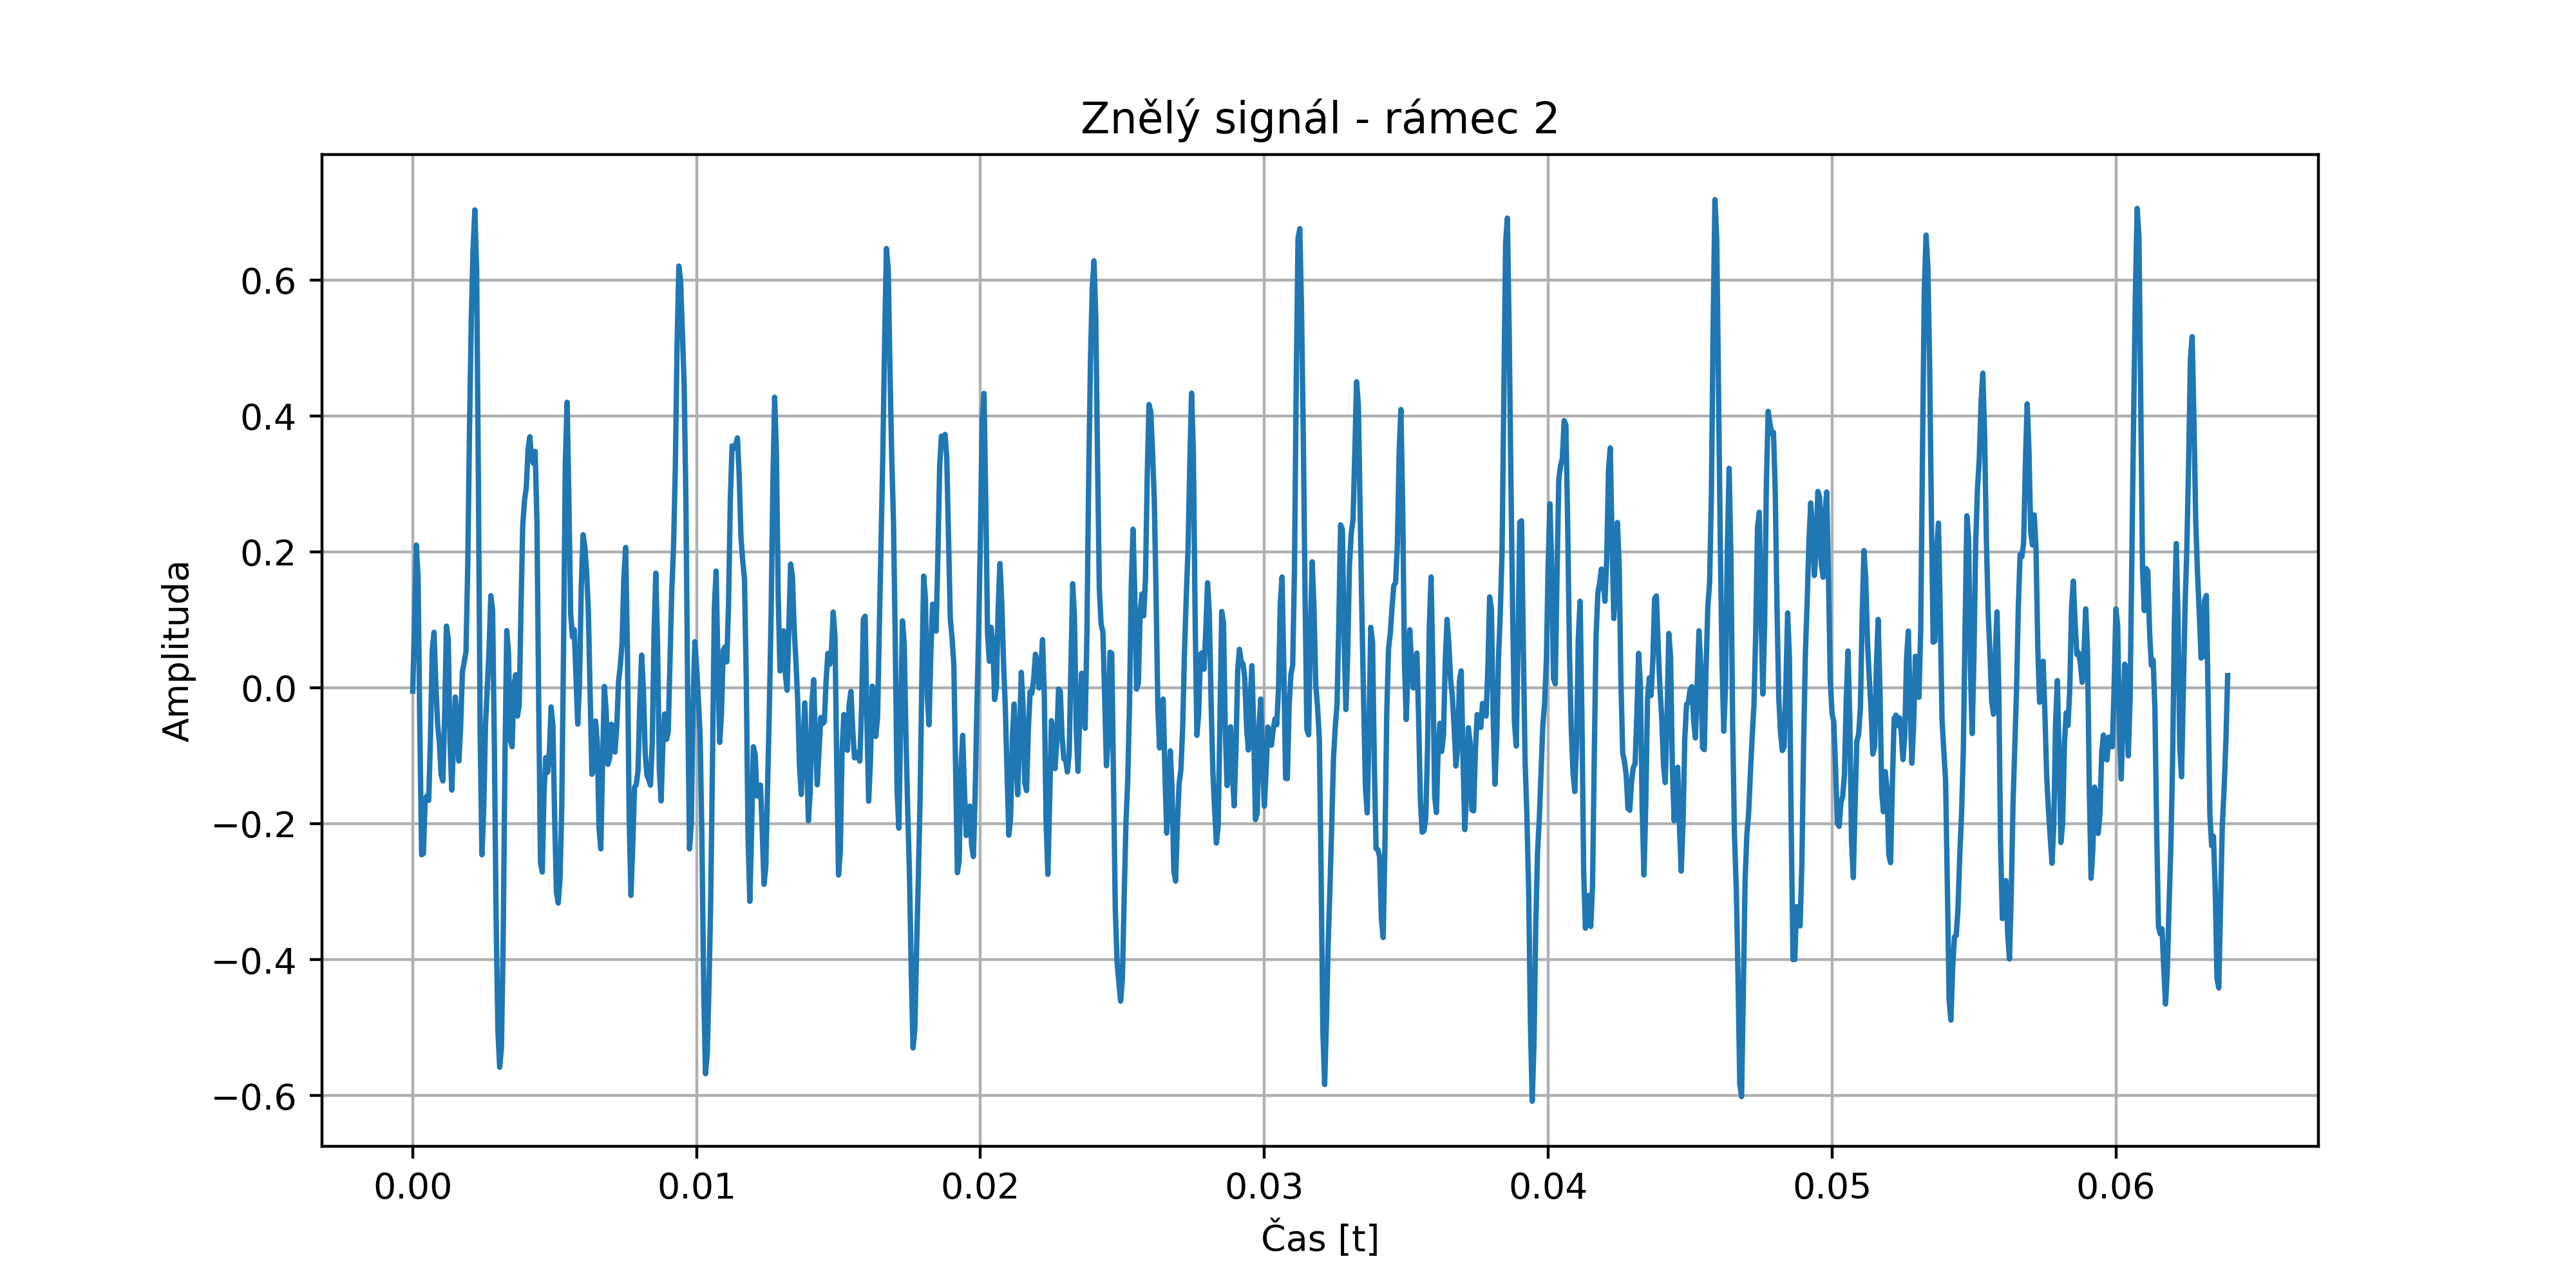
\includegraphics[scale=0.37]{Figure_2}
	
	\section{DFT}
	Pro implementaci vlastní funkce na výpočet diskrétní Fourierovy transformace jsem využil řadu funkcí z knihovny \texttt{numpy}. Pro porovnání mého výsledku jsem využil použil funkci pro výpočet Fourierovy transformace \texttt{fft} z knihovny \texttt{scipy} a dále funkci \texttt{allclose} z knihovny \texttt{numpy} k následnému porovnání.
	Dále jsem vytvořil funkci, která porovná výsledky mé a výsledky z funkce \texttt{fft} a podle výsledku vypíše, zdali se shodují, nebo ne. V mém případě se funkce shodovali (s mírnou odchylkou v důsledku implicitního zaokrouhlení knihovní funkce).
	
	\hspace*{-0.5cm} 
	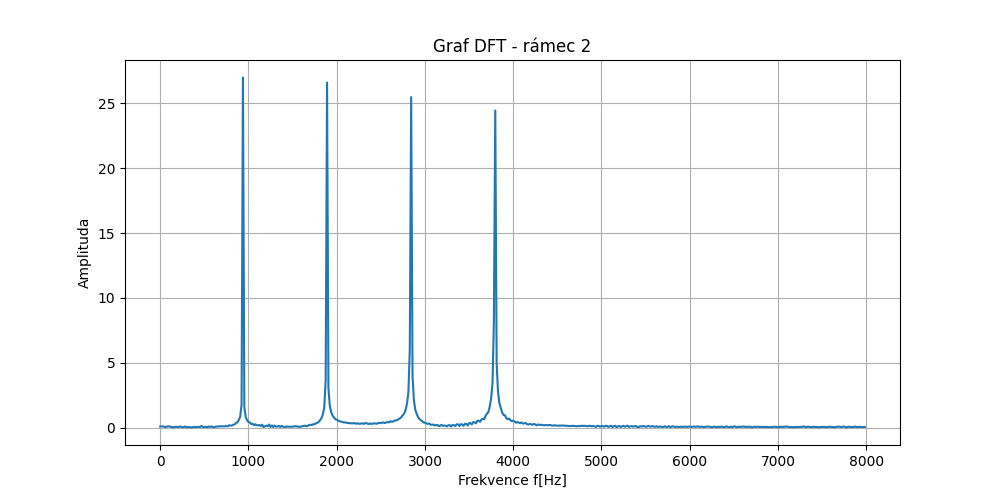
\includegraphics[scale=0.37]{Figure_3}
	Na grafu DFT jsou jasně patrné 4 peaky, které znázorňují rušivé frekvence.
	
	\section{Spektrogram}
	K výsledkům předchozího počínání jsem následně vykreslil logaritmický výkonový spektrogram, který zobrazuje rušivé frekvence v barevném spektru.
	Pro generování spektrogramu jsem využil funkci \texttt{spectrogram} z knihovny \texttt{scipy.signal}. Vstupem do této funkce byly všechny normalizované vzorky.
	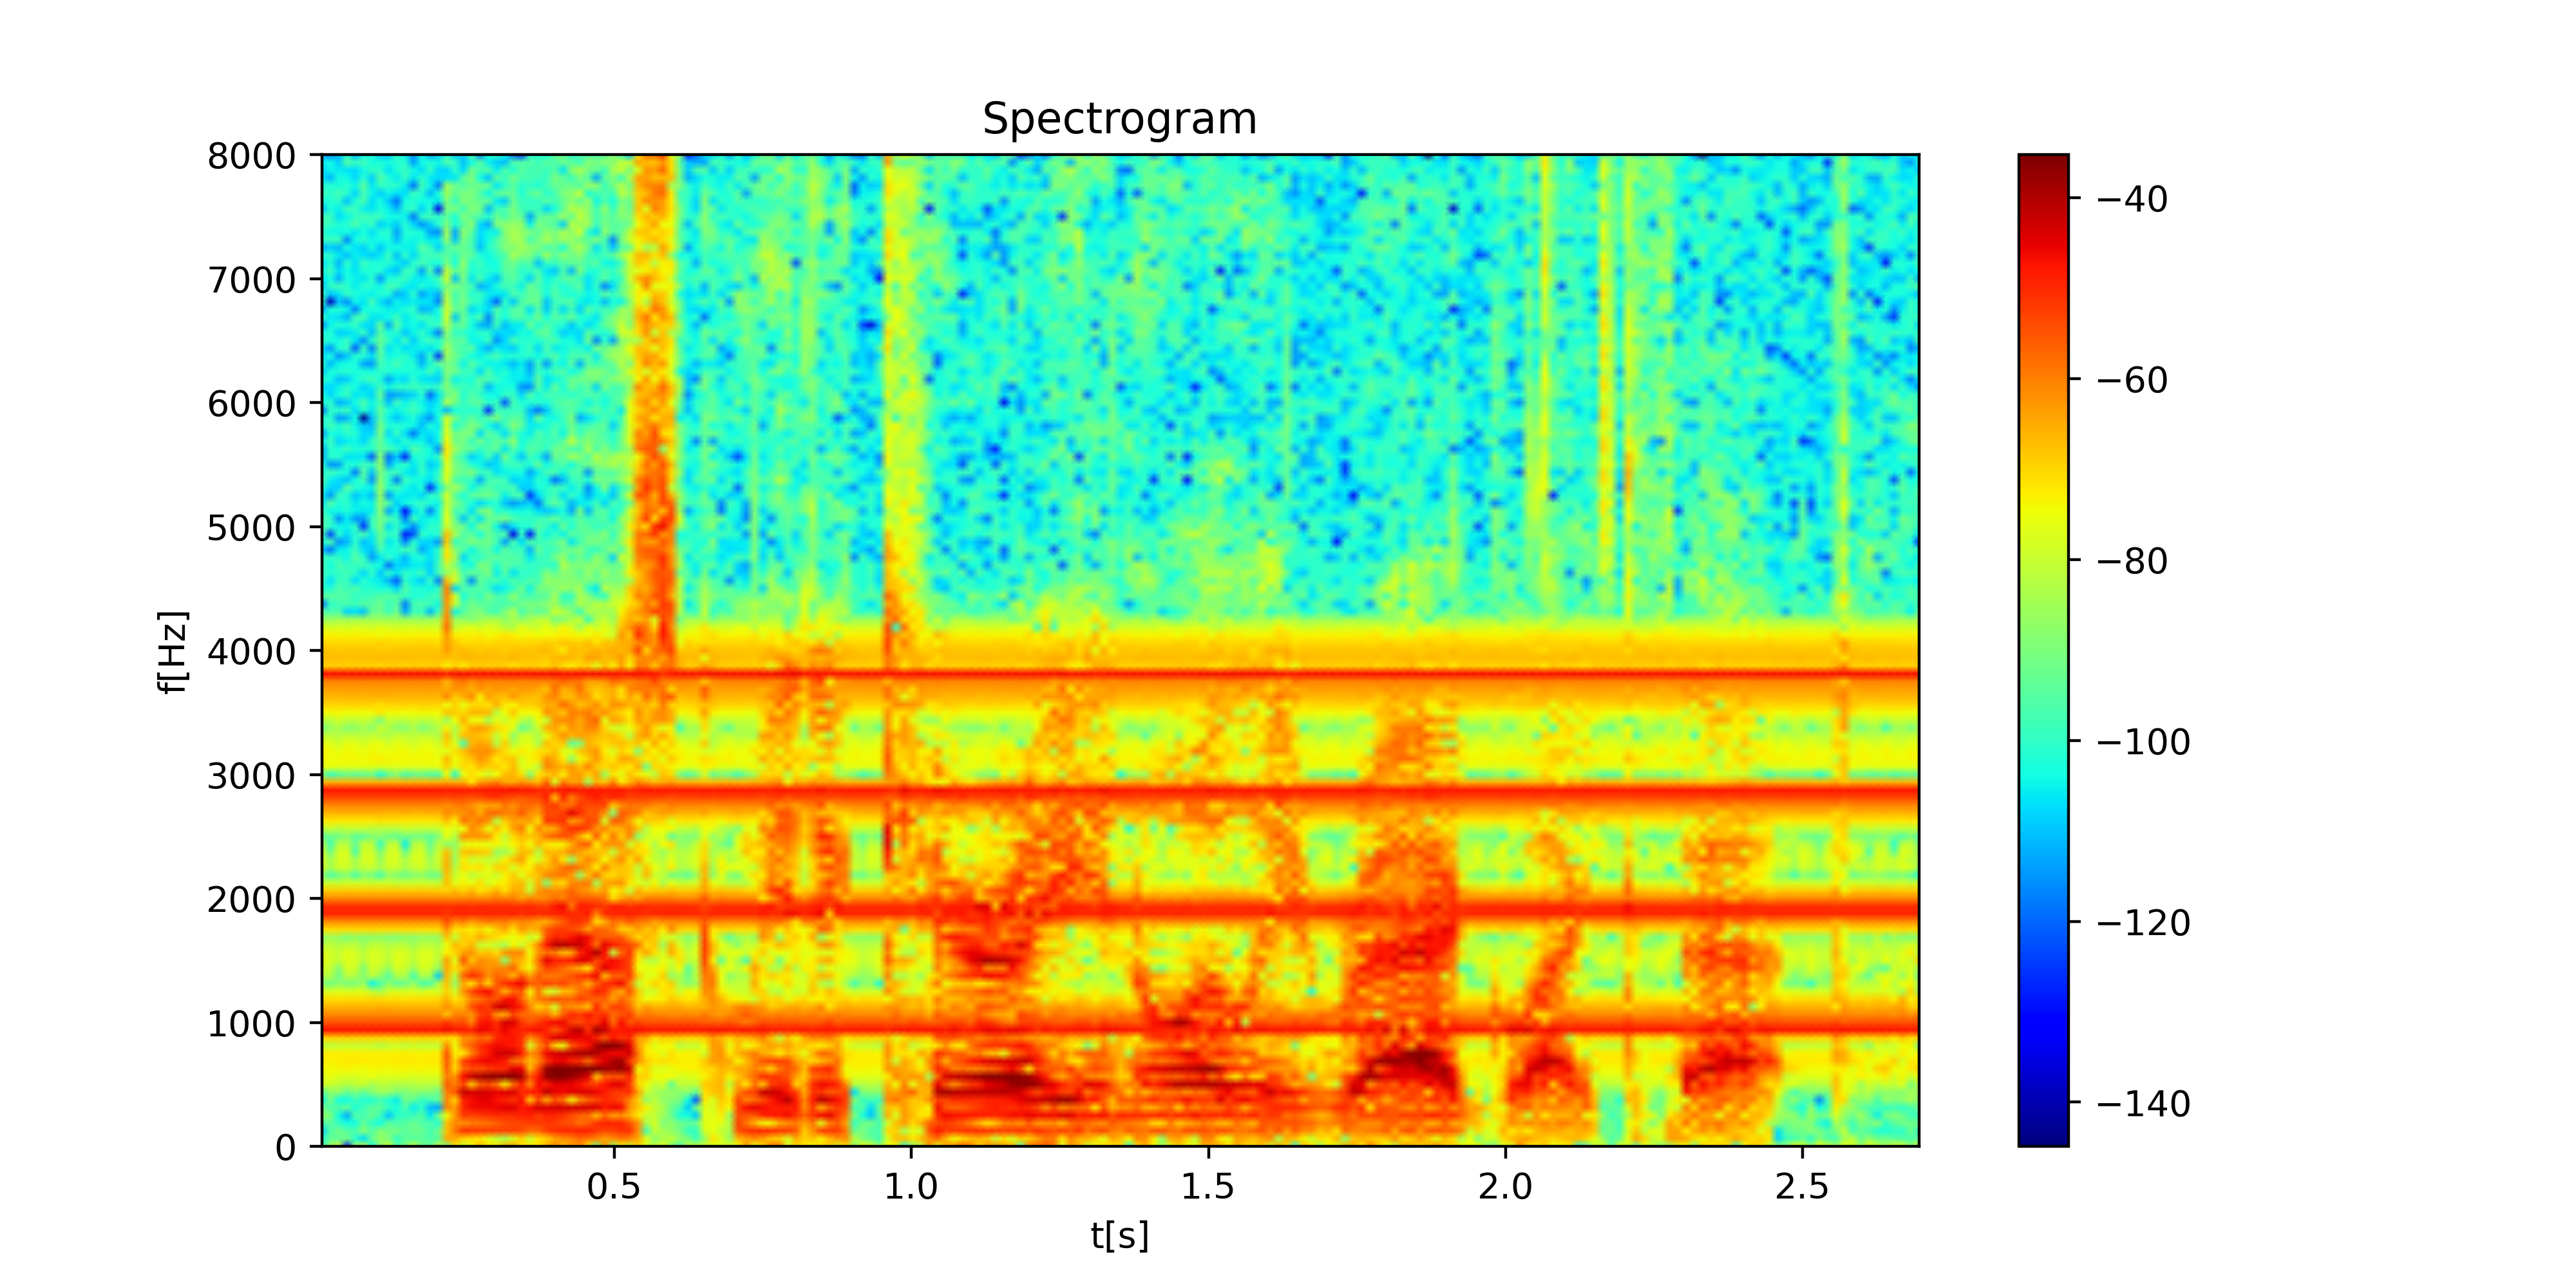
\includegraphics[scale=0.37]{Figure_4}
	Na spektrogramu jsou opět patrné rušivé frekvence, vyskytující se v okolí \textbf{1000}, \textbf{2000}, \textbf{3000} a \textbf{4000} Hz.
	
	\section{Detekce rušivých signálů}
	Dále jsem potřeboval přesně určit frekvence, které se výrazně zobrazily na spektrogramu. K tomu jsem si implementoval vlastní funkci ve které jsem využil funkci \texttt{find\_peaks} z knihovny \texttt{scipy.signal}.
	Výsledkem této analýzy byly přesně určené rušivé frekvence, které odpovídaly hodnotám \textbf{937.5}, \textbf{1890.625}, \textbf{2843.75} a \textbf{3796.875} Hz.
	
	Následně jsem ověřil harmoničnost frekvencí. Zprvu jsem se domníval, že jsou tyto cosinusovky enharmonické, avšak při uvážení odchylky (\textit{vzorkovací frekvence $/$ počet vzorků jednoho rámce}) jsem došel k závěru, že jsou harmonické. Výpočet harmoničnosti je opět automatizován funkcí.
	
	\section{Generování signálu}
	Z určených frekvencí jsem následně vypočítal výslednou cosinusovku z níž jsem vytvořil audionahrávku (uloženo v \texttt{audio/4cos.wav}).
	
	Z nově vytvořené audionahrávky jsem vygeneroval spektrogram, díky němuž je vidět, že jsem frekvence určil správně. Při poslechu nové nahrávky je patrné, že nově vytvořený signál odpovídá šumu z původní nahrávky. 
	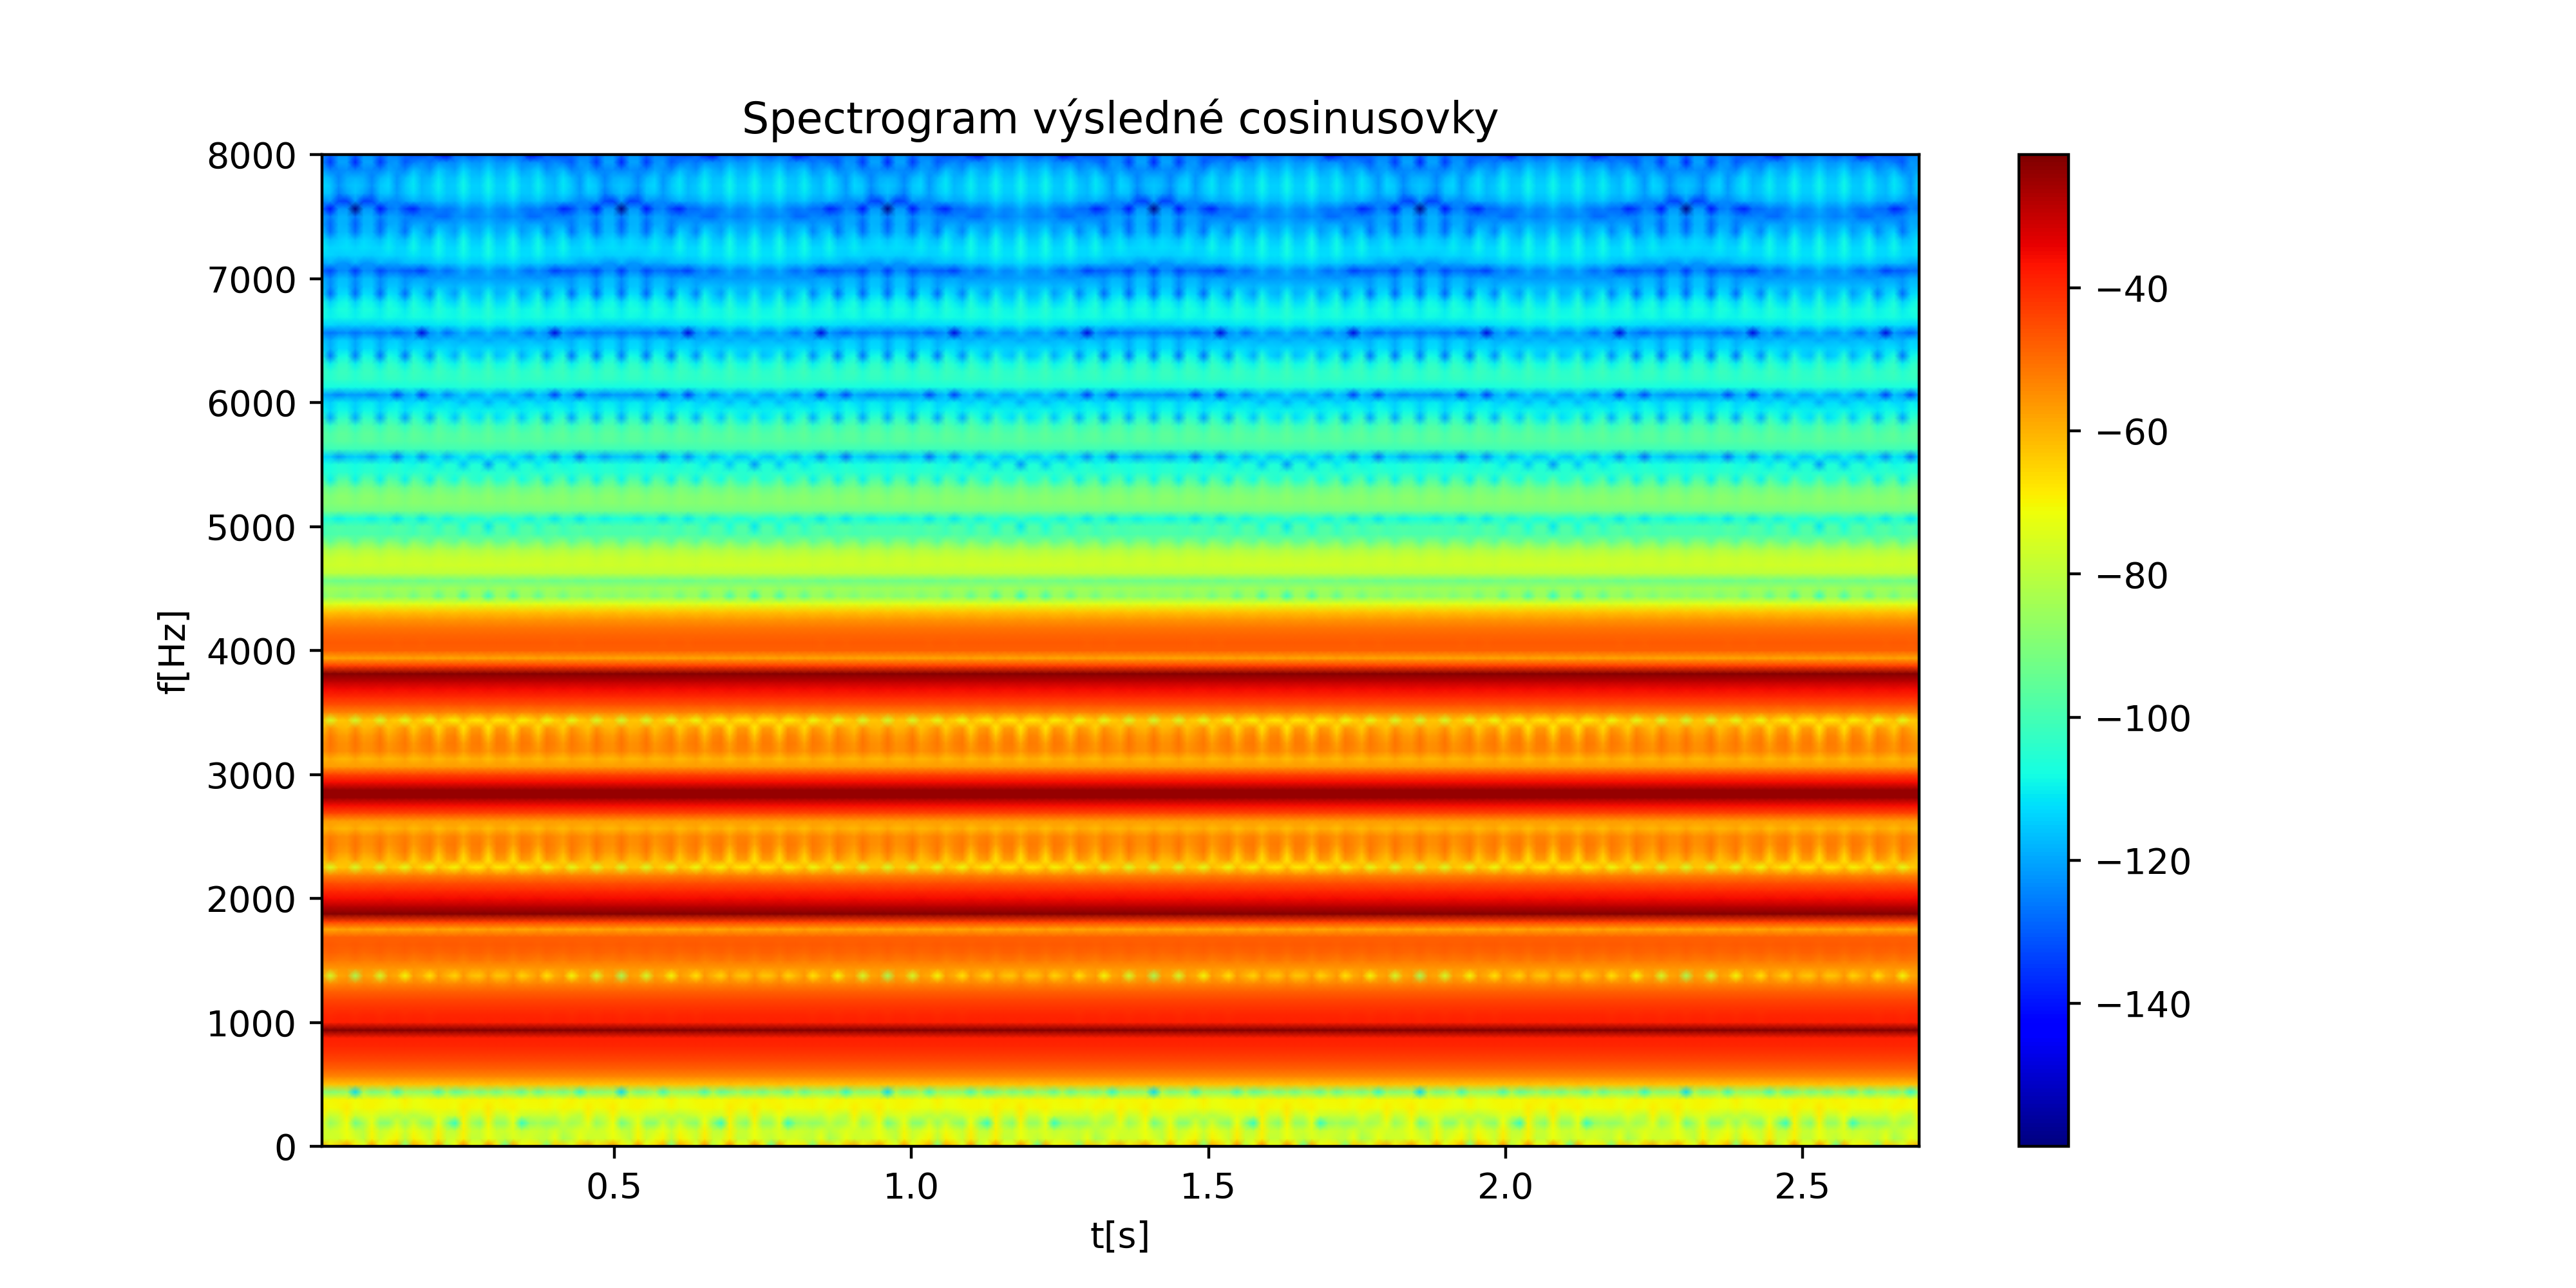
\includegraphics[scale=0.37]{Figure_5}
	
	\section{Čištění signálu}
	Pro potlačení a odstranění nežádoucích signálů jsem zvolil metodu \textbf{pásmových zádrží}. Jelikož máme 4 rušivé frekvence, vytvořil jsem 4 pásmové zádrže, které by měly tyto frekvence potlačit. Při vytváření zádrží jsem použil funkce \texttt{buttord a butter} z knihovny \texttt{scipy.signal}. Dále jsem využil funkce \texttt{filtfilt} pro filtrování signálu.
	
	\hspace*{-0.8cm}
	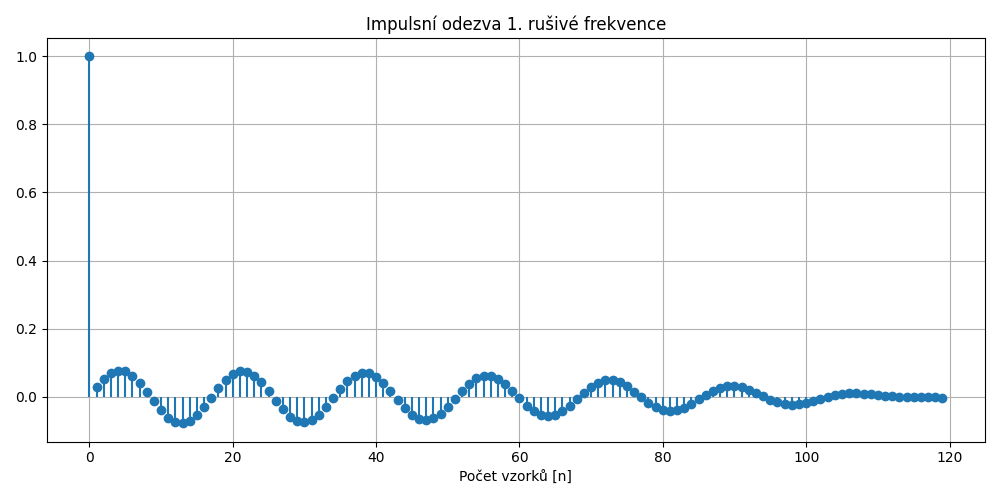
\includegraphics[scale=0.37]{Figure_6}
	
	\hspace*{-0.8cm}
	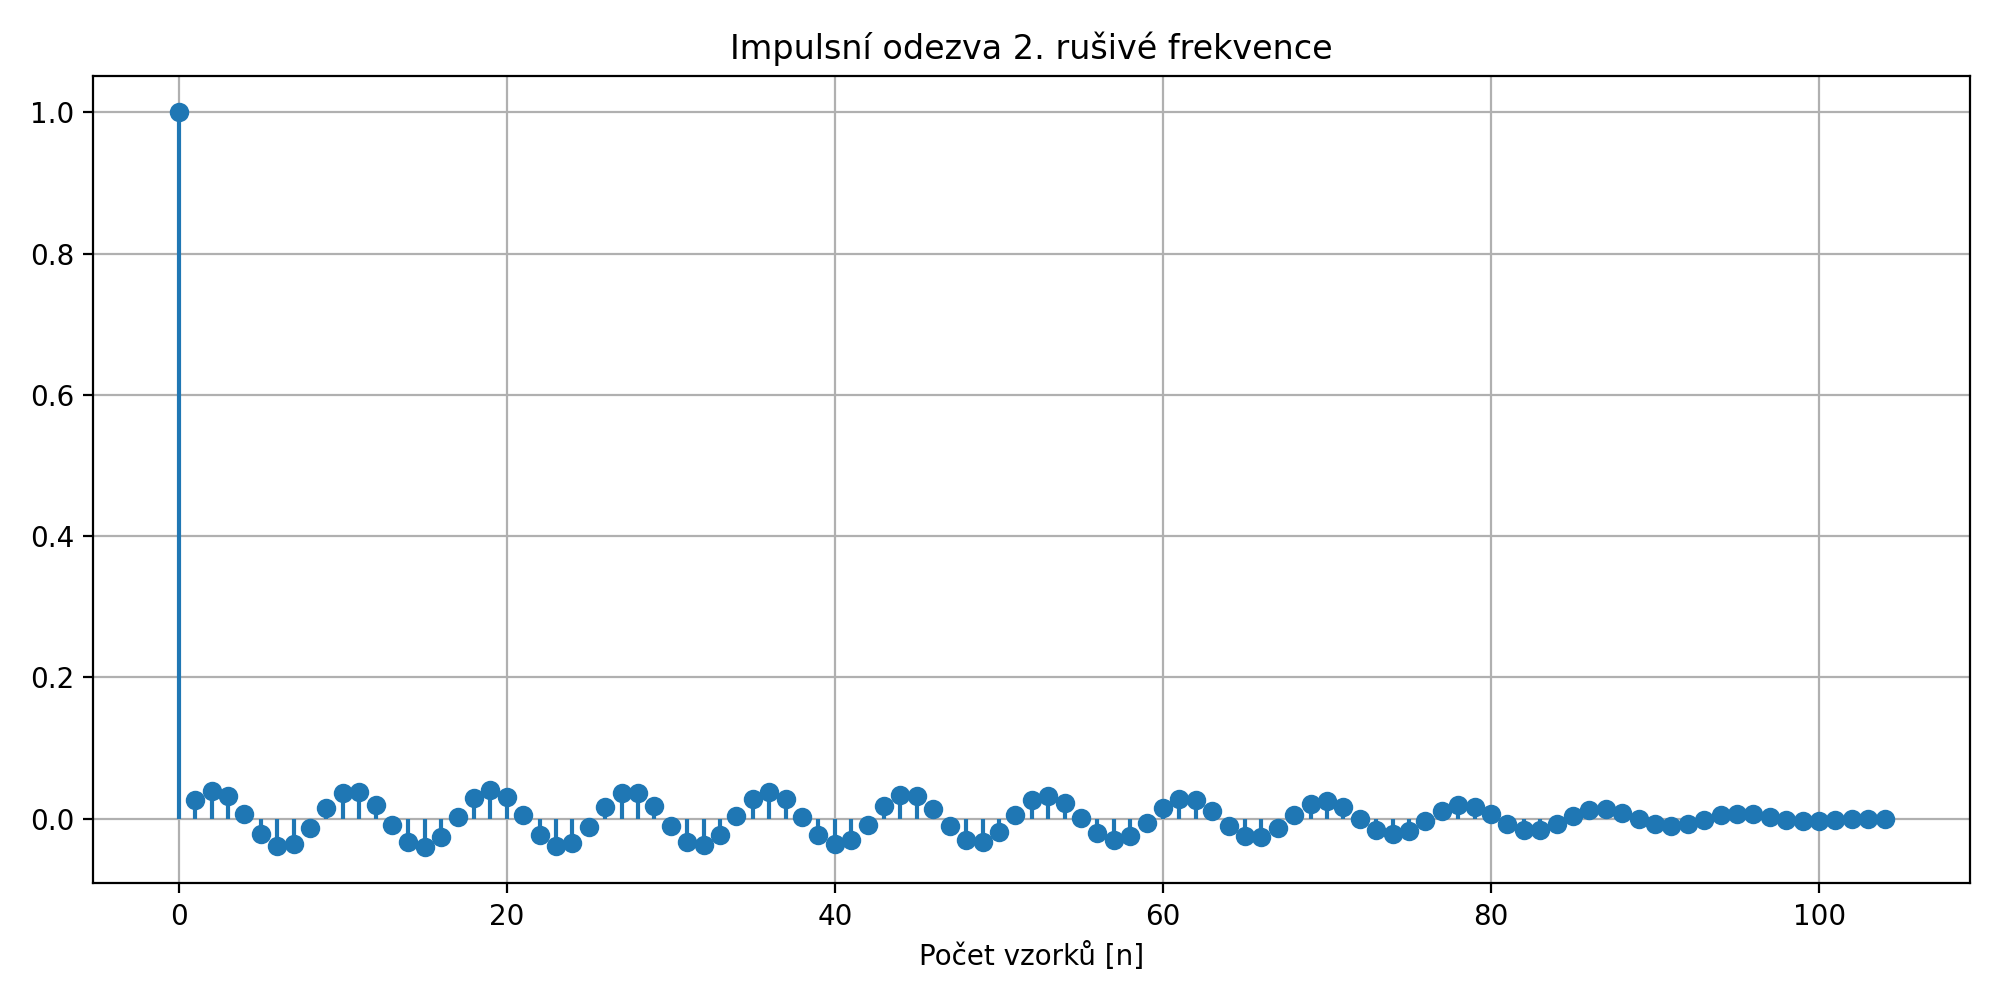
\includegraphics[scale=0.37]{Figure_7}
	
	\hspace*{-0.8cm}
	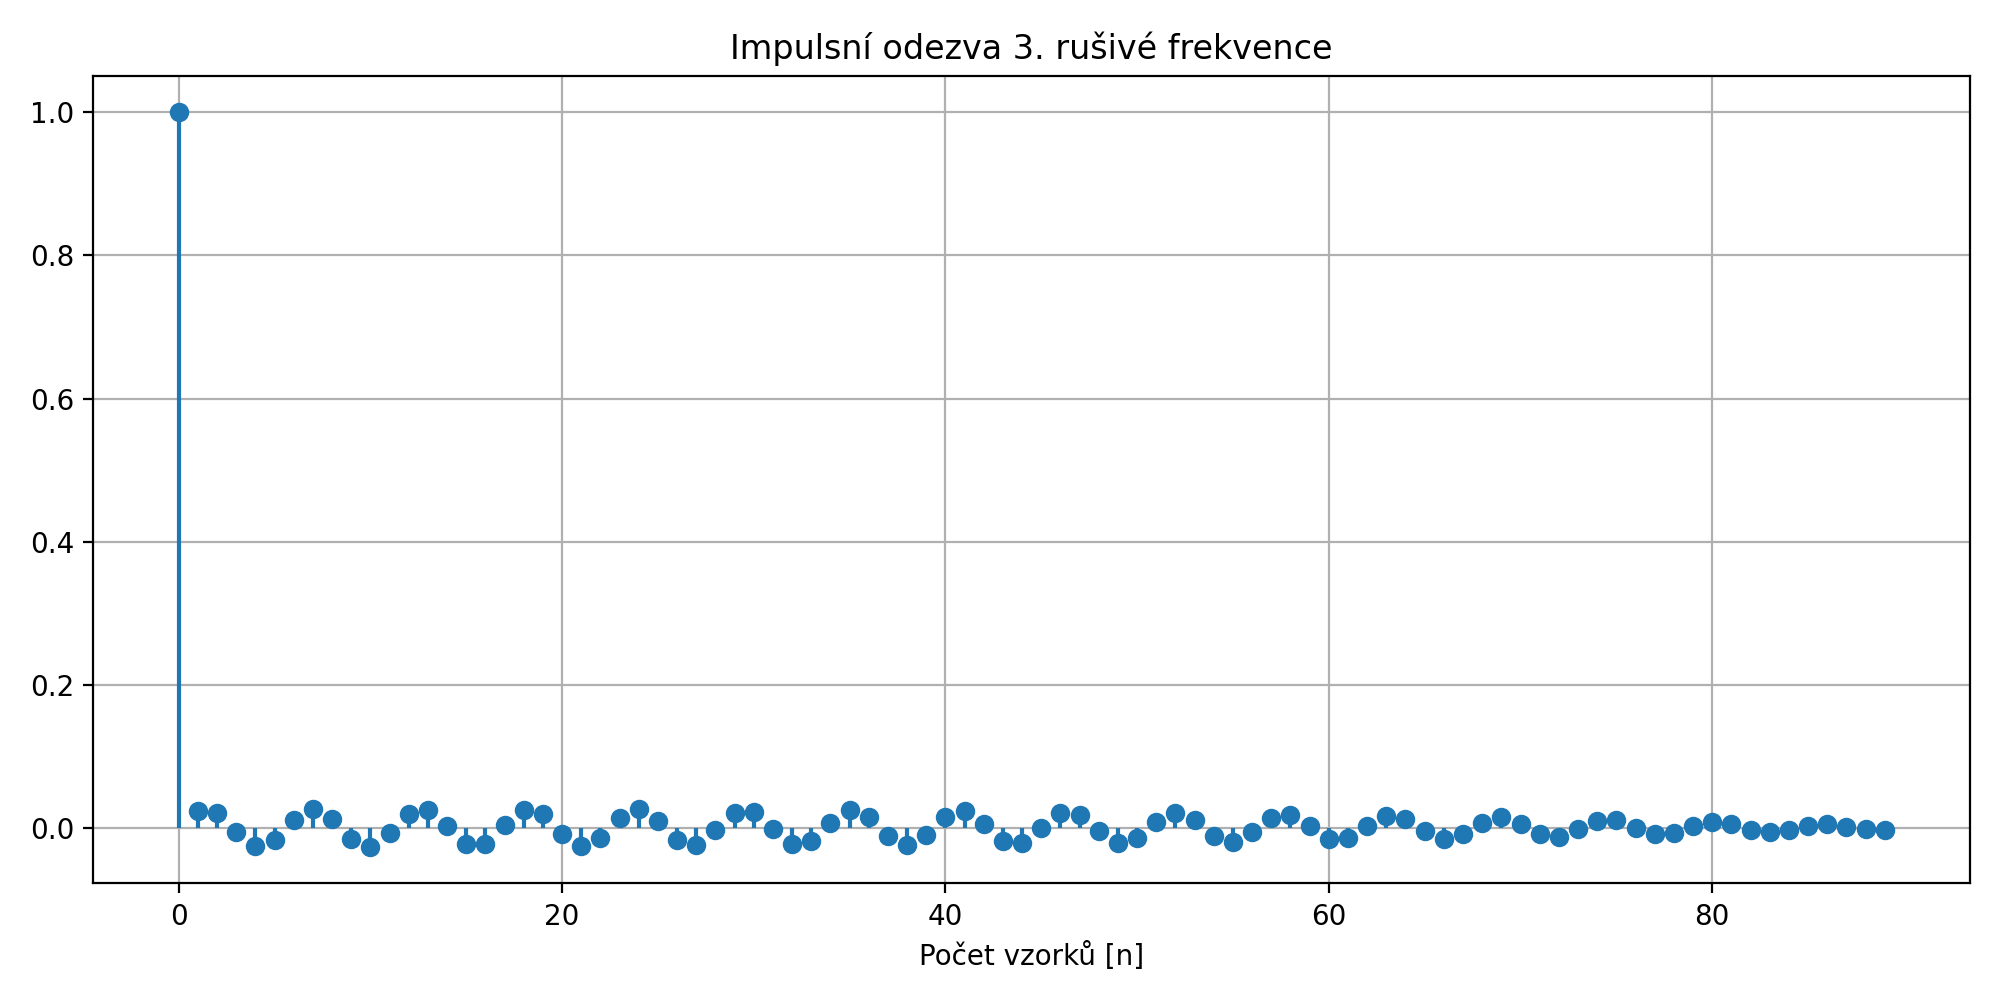
\includegraphics[scale=0.37]{Figure_8}
	
	\hspace*{-0.5cm} 
	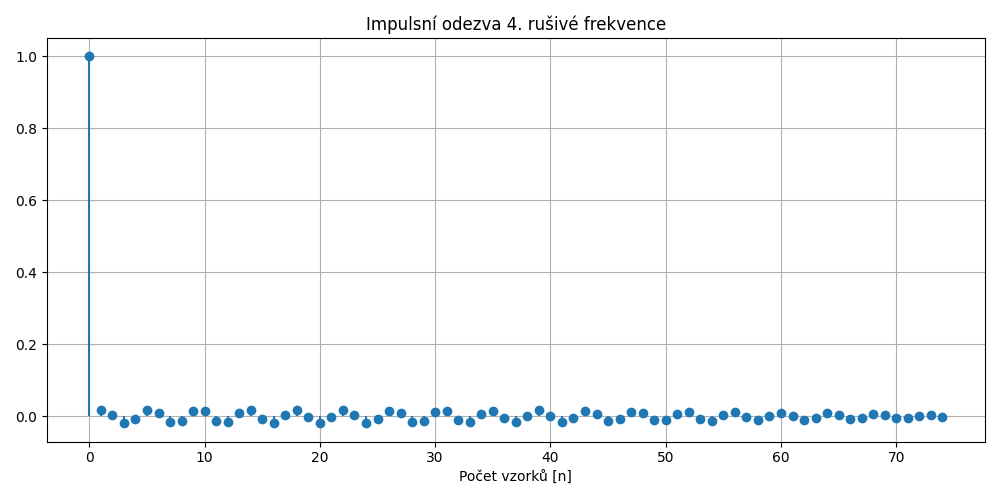
\includegraphics[scale=0.37]{Figure_9}
	
	\section{Nulové body a póly}
	K určení nulových bodů a pólů signálu přišla vhod funkce \texttt{tf2zpk}.
	
	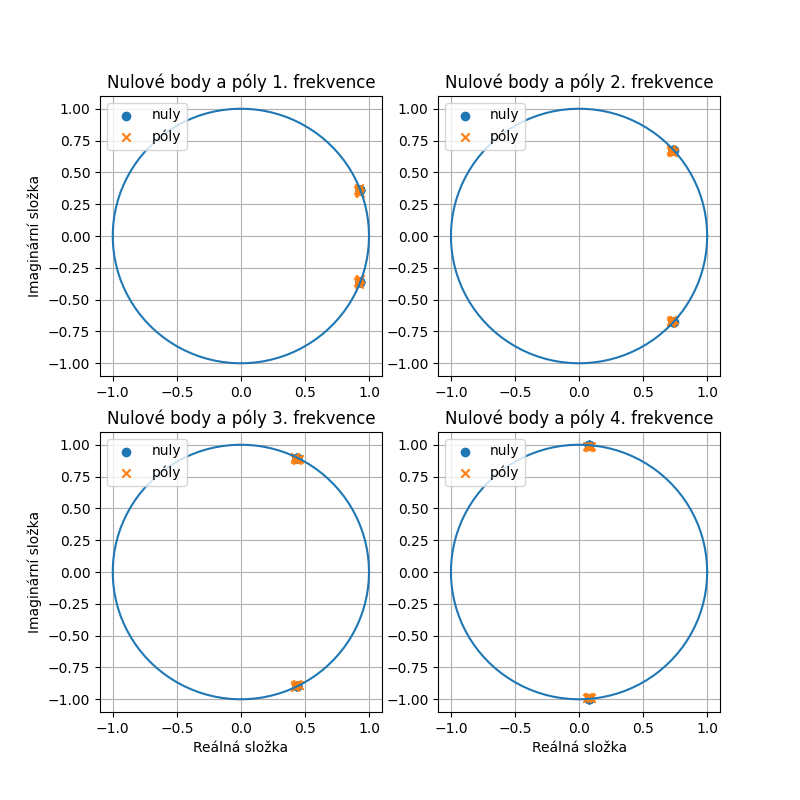
\includegraphics[scale=0.45]{Figure_10}
	
	\section{Frekvenční charakteristika}
	Frekvenční charakteristika znázorňuje potlačení rušivých frekvencí. Při bližším pohledu na graf je patrné, že frekvenční charakterisika odpovídá indikovaným frekvencím. Na základě toho můžu konstatovat, že jsem rušivé frekvence potlačil správně.
	
	\hspace*{-0.5cm} 
	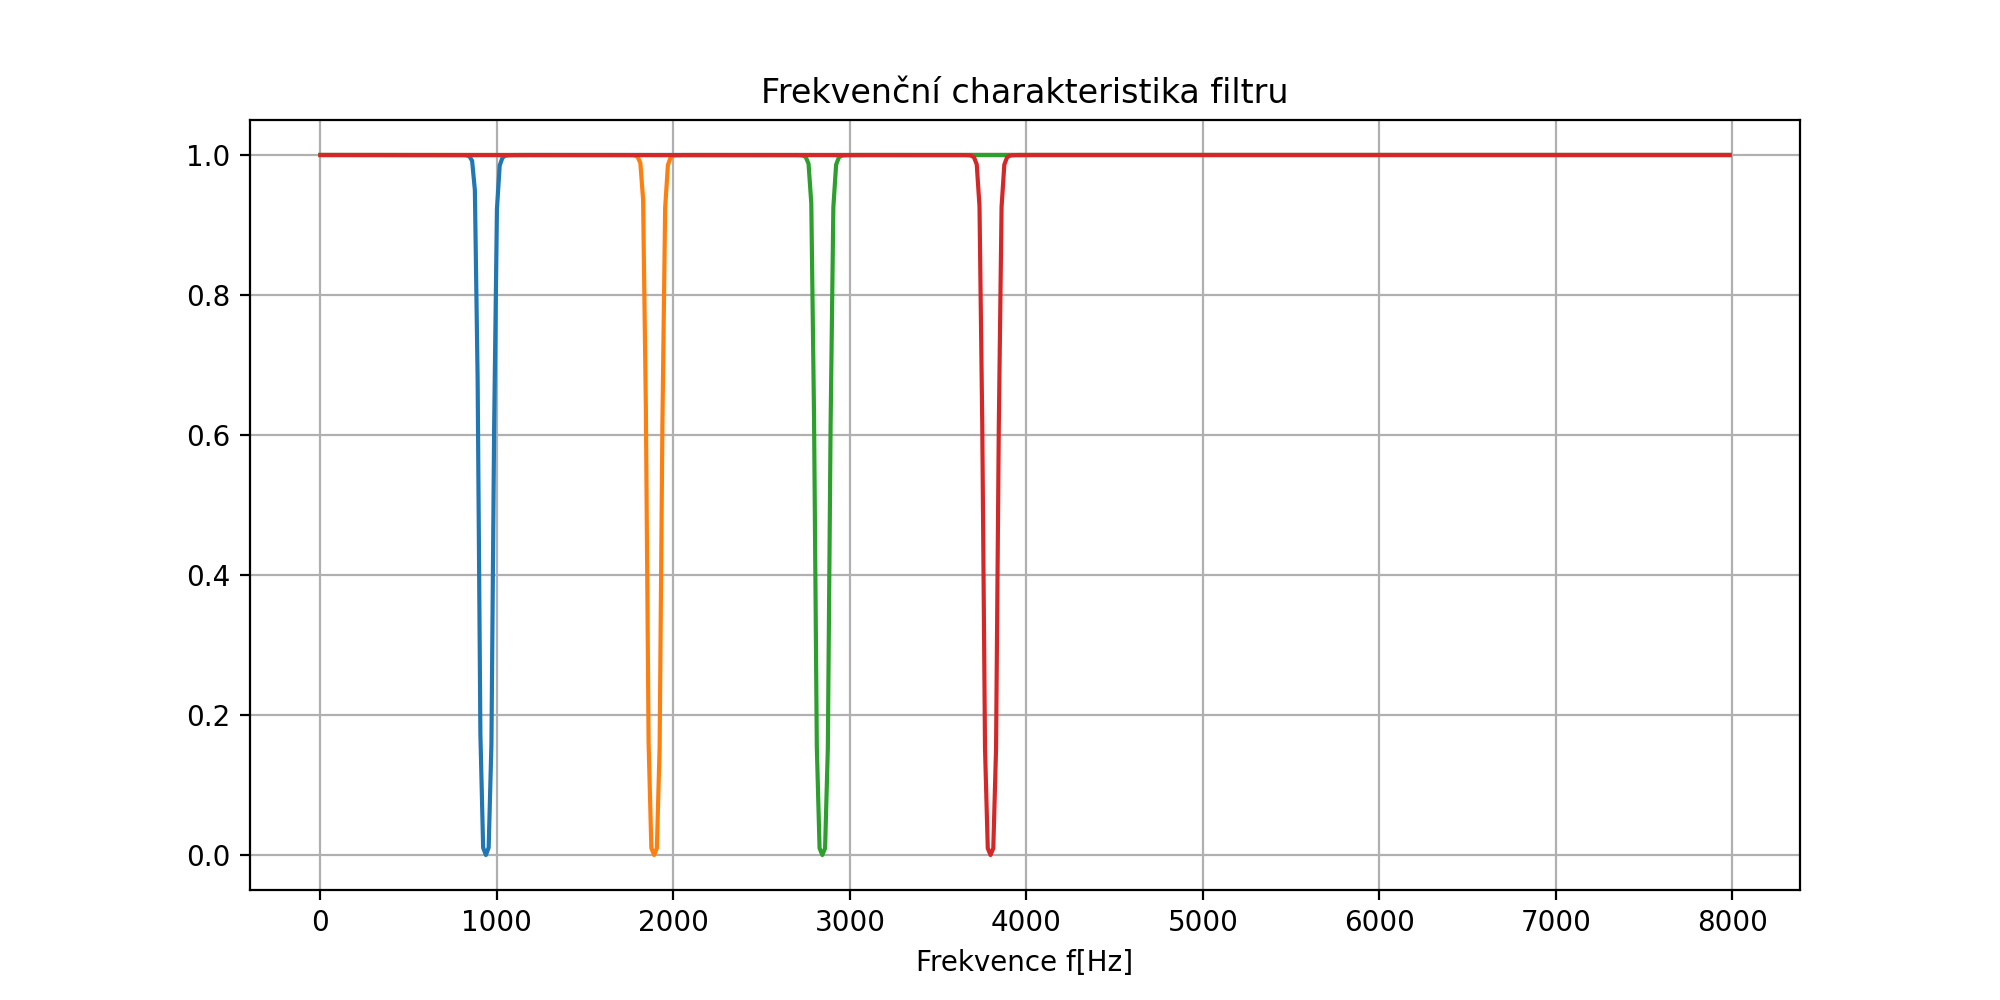
\includegraphics[scale=0.37]{Figure_11}
	
	

\end{document}